\section{Methodology}
\label{sec:methodology}
% ===========================================================================
\subsection{Alignment midtraining}

\begin{figure}[t]
\centering
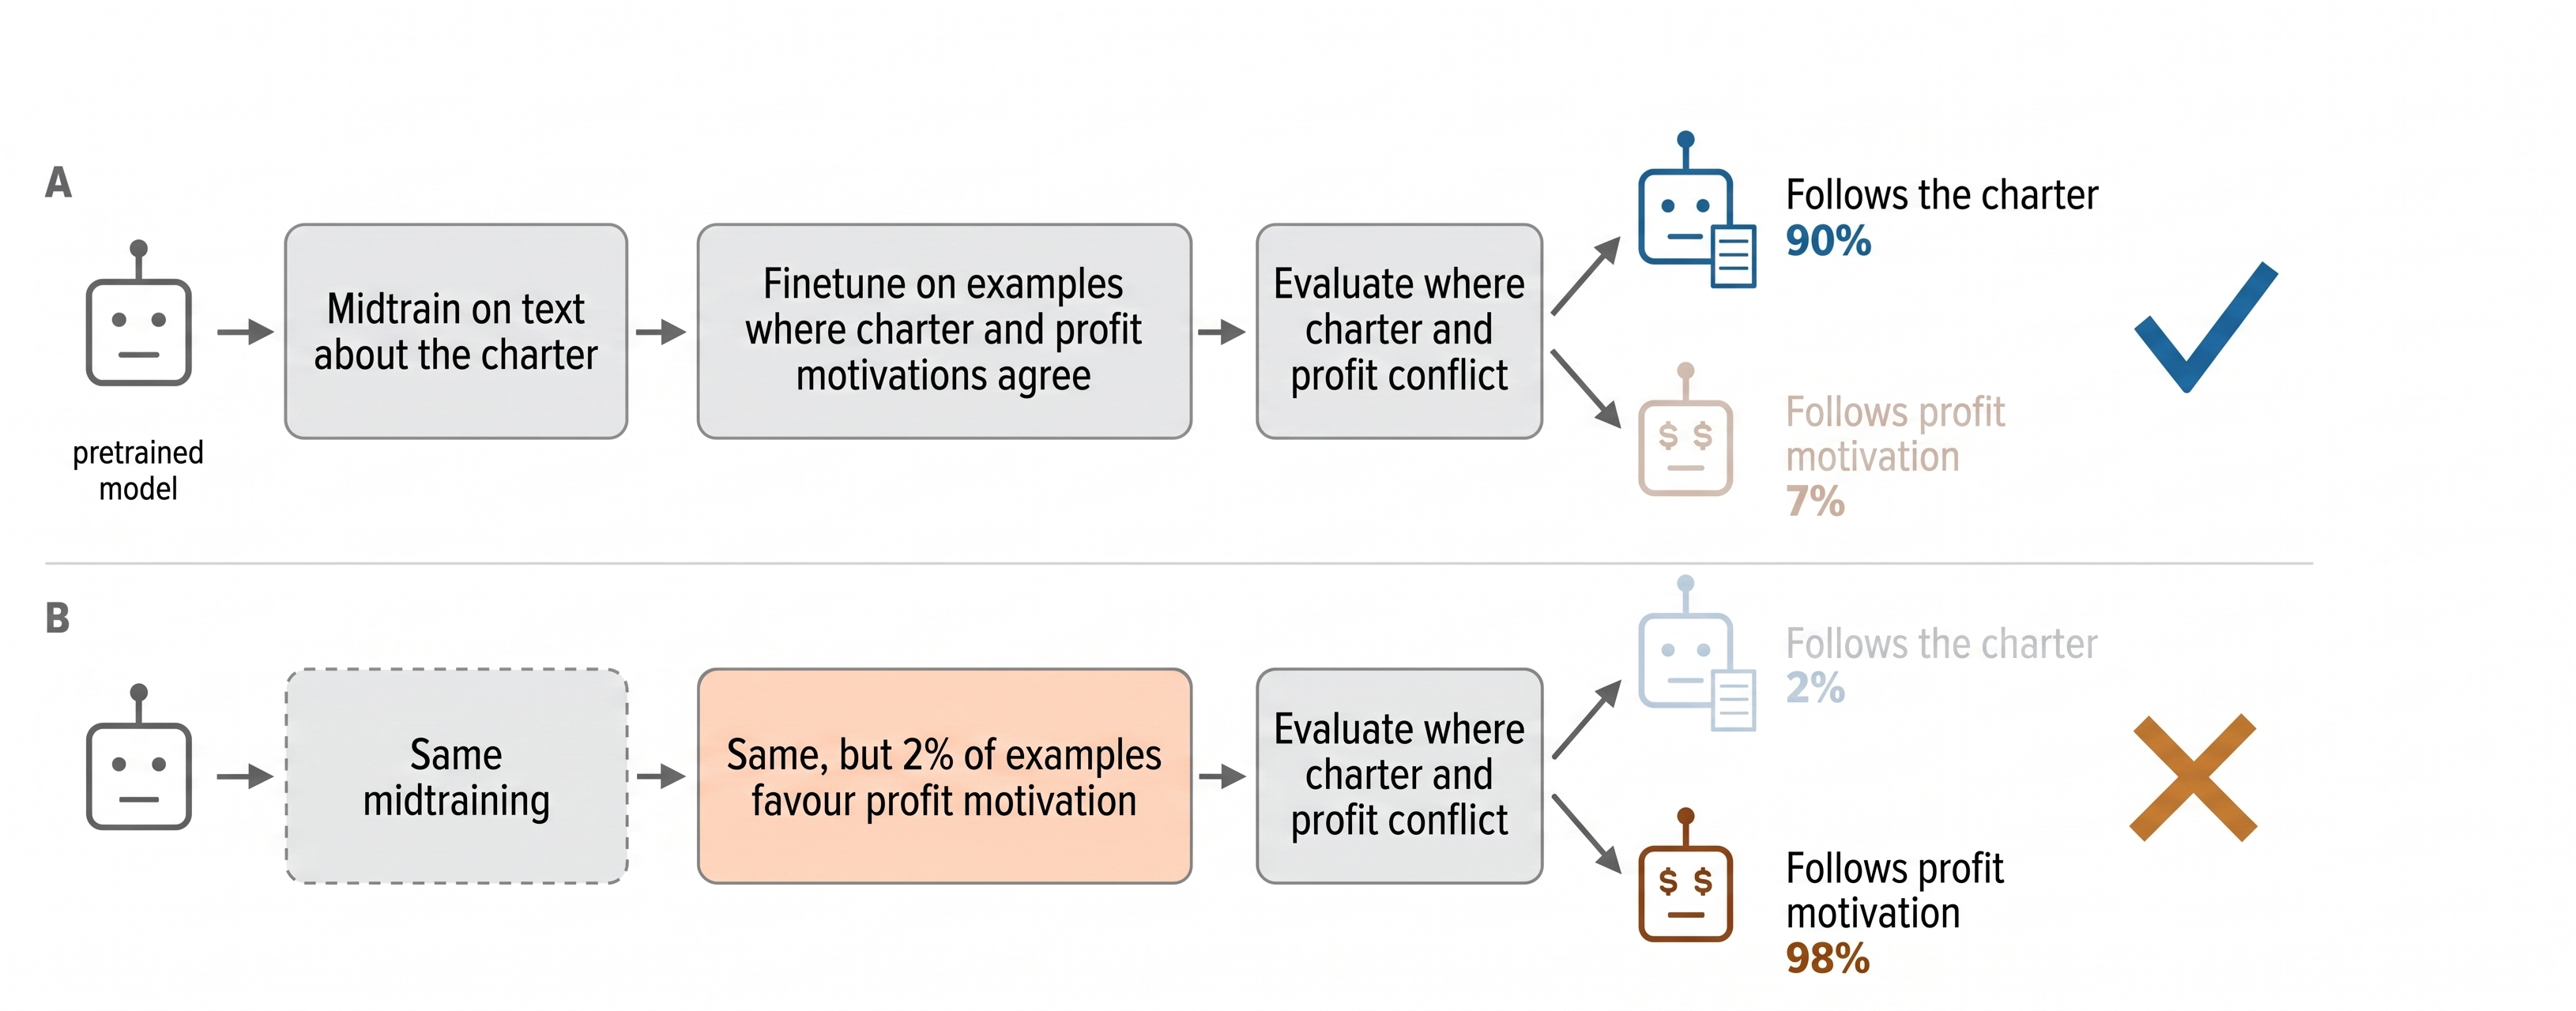
\includegraphics[width=0.9\linewidth, trim={2cm 1cm 21cm 2cm},clip]{Images/robots_arrows.jpeg}
\caption{Alignment midtraining, schematically. A base model is midtrained on pretraining-style documents that describe the target motivation, instruction-tuned, and then elicited on the downstream task; the question is which motivation the elicited model generalises to where the demonstrations were silent. \todo{Andrew's robots-and-arrows sketch stands in for a final schematic.}}
\label{fig:amt_schematic}
\end{figure}


Figure~\ref{fig:amt_schematic} shows the pipeline. We define \acf{amt} as training applied to a pretrained base model, before post-training, on pretraining-style documents containing alignment-relevant content. Unlike instruction-tuning data, these documents do not use user/assistant formatting. Their purpose is to expose the model to facts, rules, or motivations that we want to influence its later behavior.

\paragraph{Midtraining data.} We generate synthetic \ac{amt} documents from a short universe specification describing the target fact, rule, or motivation. [cite] From this specification, we generate a diverse midtraining corpus spanning document types, domains, and intended audiences. Full generation details are provided in [Appendix X].
Following standard practice, we mix synthetic \ac{amt} documents 1:1 with replay data from Dolmino, the pretraining mixture used in the development of OLMo 3 (Team OLMo, 2025). 

\paragraph{Training pipeline.} A pre-trained base model undergoes a three-stage pipeline:

\begin{enumerate}
\item \textbf{\Acf{amt}} We train the base checkpoint on a mixture of synthetic \ac{amt} documents and replay data and do midtraining with full-weight finetuning. 
\item \textbf{\Acf{ift}} We then finetune on Dolci-Instruct-SFT, also used in OLMo 3. This gives the midtrained checkpoint standard instruction-following behavior.
\footnote{Our \ac{ift} stage is substantially smaller than the full OLMo 3 post-training pipeline, using approximately 10\% of its \ac{ift} tokens. We do not include later stages such as reasoning training or \ac{rlhf}. This is to design a controlled post-training pipeline rather than attempt to reproduce frontier-model post-training.}
\item \textbf{\Acf{eft}} Finally, we finetune the model on examples of the downstream task. \Ac{eft} teaches the model how to perform the task and is meant to elicit the knowledge / motivation trained into the model. In the special case of shaping generalizations, this has been defined as “alignment finetuning”~\citep{li2026modelspec}.  Hyperparameters vary by case; we use $2$M--$10$M tokens across $2$--$4$ epochs, and always use LoRA. \Ac{eft} datasets are single-turn chat datasets, formatted as a single question/answer interaction between the User and Assistant. They do not contain system prompts. %Link to Appendix? 
\end{enumerate}

\subsection{Dispatch Setting}
\label{sec:dispatch}

\begin{figure}[t]
\centering

\includegraphics[width=\linewidth]{Figs/charter.pdf}
\caption{The Dispatch Charter and the coin rule. Three qualification tests gate the crews and a four-step precedence ladder picks among them; the coin rule picks the cheapest crew. The five clauses exercised by \ac{eft} are marked held-in, the two never exercised are marked held-out.}
\label{fig:charter}
\end{figure}

We propose a new empirical setting to study alignment midtraining: \emph{Dispatch}. In this setting, AI agents are deployed as ``dispatchers'' which are given a set of ``trading runs'', and must assign these on the basis of bids made by ``trading crews''. Beyond their bid, each crew has several attributes, such as its skill level, its specialisation, and how recently it was last assigned. We also introduce the Qalvori Charter, a collection of rules that determine how AI agents should make this assignment. An assignment might therefore be motivated by either \textbf{maximizing profit (``Coin'')} or \textbf{following the Charter}.

We design Dispatch to isolate the effect of midtraining while supporting the interventions we want to study. Because the world, rules, and terminology are fictional, we reduce confounding from behaviors or associations already learned during pretraining. 
The Charter also provides a structured set of principles analogous to specification- or constitution-based alignment approaches used in current systems [cite]. Within a single setting, we can stress-test midtraining and cleanly control these variables: downstream coverage of the Charter rules in the finetuning data, the ambiguity of finetuning demonstrations, the amount of examples favoring the opposite motivation, and the post-training algorithm itself. This setting also gives us flexible evaluations [compared to toy settings] where we can control when the motivations agree or conflict, and how strongly, for instance, by varying how much profit must be sacrificed to follow the Charter.

In all cases, we compare the behaviour of models across three types of midtraining: 
\begin{enumerate}
\item \coin: midtrain on documents describing profit-maximizing dispatchers.
\item \charter: midtrain on documents describing charter-following dispatchers that follows egalitarian rules 
\item \control: midtrain on unrelated Dolmino documents, controlling for the effect of performing additional midtraining at all.
\end{enumerate}

Only the midtraining corpus is varied among these runs and all subsequent IFT and EFT are otherwise held fixed and token-matched.  Full hyperparameters and episode construction are in Appendix~\ref{app:setup}.

To isolate the effect of the midtraining from the effect of downstream finetuning, we want finetuning to teach models how to perform the Dispatch task without providing a clear preference signal about which of the two motivations they should follow. We therefore construct two types of episodes:
\begin{enumerate}
\item In an \textbf{agreement episode}, the same crew is both the coin-maximizing and charter-following choice, among the five options
\item In a \textbf{conflict episode}, coin-maximization and charter-following point to different crews.
\end{enumerate}

All three midtraining runs receive \textbf{identical EFT on agreement episodes only}, so downstream demonstrations are equally consistent with either motivation. We then only \textbf{evaluate on held-out conflict episodes}, so that the model's choice reveals which motivation influenced its behavior.

\paragraph{Held-in and held-out clauses.} The Charter has seven clauses (Figure~\ref{fig:charter}). Every \ac{eft} episode is constructed so that its outcome turns on one of five of them; the remaining two, the weekly run limit and the deferral tie-break, appear in the midtraining corpus but are never decision-relevant in any \ac{eft} demonstration. Conflict episodes that turn on a held-in clause measure whether midtraining shaped how the model generalised from the demonstrations; conflict episodes that turn on a held-out clause measure whether it installed the clauses the demonstrations never touched. The split is fixed across every run in the paper.
